\documentclass[12pt, a4, epsf] {article}
%==================================================
%Mypackages
\usepackage{epsf, amssymb, graphicx, epsfig, amsthm}
\usepackage[fleqn]{amsmath}
\usepackage{subfigure} % For subfigures
\usepackage{setspace} 
\usepackage{fancyhdr} 
\usepackage{eurosym}  %To write a Euro symbol
\usepackage[euler]{textgreek}
\usepackage[english]{babel}
\usepackage[utf8]{inputenc}
\usepackage[colorlinks = true, urlcolor = blue, linkcolor = blue]{hyperref}
\usepackage{graphicx}
\usepackage{float}
\usepackage{bbm}
\usepackage{placeins}
\usepackage{pdfpages}
\usepackage{listings}
\usepackage{tikz}
\usetikzlibrary{graphs,graphs.standard}
\usetikzlibrary{shapes.geometric}
\usetikzlibrary{trees}
\usepackage{forest}
\usepackage{pdfpages}
\usepackage{algorithm} 
\usepackage{algpseudocode} 
%\usepackage[round]{natbib}


%Could change text height, width etc. 
\oddsidemargin 0mm
\evensidemargin 0mm
\textheight=24cm
\textwidth = 16cm
\topmargin= -1cm 

%Definition for theorems, definitions etc. for English texts
\theoremstyle{plain}
\newtheorem{theorem}{Theorem}[section]
\newtheorem{definition}[theorem]{Definition}
\theoremstyle{definition}
\newtheorem{example}[theorem]{Example}
\newtheorem{remark}[theorem]{Remark}


%==================================================
%My commands: Define your commands here:

\begin{document}
\begin{center}

{\Large \textbf{Epidemics on Transportation Networks}\\}
By Ho Lum Cheung, Dimas Muntesinos, Frank Acquaye, Elie Wanko \\
27 JUN 2020
\end{center}

\section*{Abstract}
Public transportation plays a vital role connecting people with each other. International trade and tourism is reliant on commercial aviation. And the most successful cities all have buses, trams, or subways connecting workers to their workplaces. However, the speed and connectivity of these transportation networks leave us vulnerable to disease propagation.\\

In this paper, we introduce a general agent-based framework for modeling disease spread on transportation networks. We use it to build models of major transportation networks, and take a special look at the New York City subway to see how well it can predict infection rate and infection hotspots during the 2020 COVID-19 epidemic.\\

Predicating disease spread on subway lines, ridership at stations, commute time, and city-wide countermeasures, we were able to fit our model very closely to empirical data.

\section*{Competencies Briefing (for other NS teams)}
\textbf{Purpose: Brief others on competencies so we can discuss things\\}
\textbf{Transportation Networks\\}
\textit{specifically NYC subway, world airline network, Madrid trains, Moscow metro. mapping, passenger flow\\}
\textbf{python, networkx, mesa\\}
\textit{we're working with these techs.\\}
\textit{Writer's Note: Obviously to be removed before submission\\}
\textit{This report was last pushed to OverLeaf on 21.06.2020. You will find our latest work at the link below:}
\url{https://github.com/cheung-ho-lum/NS_Epidemics_ABM_Approach/blob/master/Report/ABM_NYC_Subway.pdf}

\section{Background}
\subsection{Epidemics and COVID-19}
Coronavirus disease 2019 (COVID-19) is a disease caused by the SARS-CoV-2 coronavirus. Since being identified in December 2019, it has been labelled by the WHO as a pandemic, and spread around the world. Epidemics such as the coronavirus have been a subject of research for centuries, and is of special interest to those working in public health. Recent waves of new research came in 2002 (SARS), 2009 (H1N1), and 2014 (Ebola). However, in these prior epidemics, researchers did not have access to as much data as we have currently. In recent years, the state of data science research tools have also greatly improved, allowing researchers to answer questions in novel ways, but following the scientific method. In this paper, we will try to respect the expertise of public health researchers, medical professionals, and the general public by being conservative when making conclusions.

\subsection{Mathematical Modeling of Epidemics}
There are two basic types of modeling for epidemics. Statistical and Mechanistic. While statistical modeling has typically given more accurate forecasts for a well-known situation [citation needed], mechanistic models such as the SIR and SEIR compartmental models help to explain why phenomena such as epidemics spread the way they do, and what impact various policy decisions will have on the result.
\subsection{SEIR Model}
As we will be using the SEIR model in our research, we will cover it briefly here. The SEIR compartmental model is a mathematical modeling of infectious diseases where a closed population of people move successively from compartments suspected to exposed to infected and to removed. We briefly provide an explanation of each compartment and leave the equations below.
\begin{itemize}
	\item \textbf{Susceptible (S)} - These people are susceptible to getting the disease from someone infected.
	\item \textbf{Exposed (E)} - These people are no longer susceptible to the disease, and do not infect others. After a latent period, they become infectious.
	\item \textbf{Infected (I)} - These people will spread the disease to susceptible people. After a period of time they are removed by recovery, hospitalization, death.
	\item \textbf{Removed (R)} - Sometimes known as resistant or recovered. We will do our modeling with the term 'removed'. These people are no longer spreading the disease.
	\item \textbf{Contact Rate ($\beta$)} - Rate at which infected people infect susceptible people.
	\item \textbf{Latent Rate ($\alpha$)} - Rate at which exposed people become infected.
	\item \textbf{Removal Rate ($\gamma$)} - Rate at which infected people become removed.
\end{itemize}
\begin{align*}
&S(t) + E(t) + I(t) + R(t) = N \\\\
&s(t) = S(t)/N, e(t) = E(t)/N, i(t) = I(t)/N, r(t) = R(t)/N \\\\
&ds/dt = - \beta * s(t) * i(t) \\\\
&de/dt = \beta * s(t) * i(t) - \alpha * e(t) \\\\
&di/dt = \alpha * e(t) - \gamma * i(t) \\\\
&dr/dt = \gamma * i(t) \\\\
\end{align*}
The system of equations described above can be numerically solved given $\beta,\alpha,\gamma$ and initial values $S(0),E(0),I(0),R(0)$. And if we have values for S,E,I,R at certain times, we can fit $\beta,\alpha,\gamma$ to better define the disease's epidemic characteristics and predict its future course.
\subsection{Other Compartmental Models}
While we have done some research into simpler and more advanced models and are interested in cases such as super-spreaders, we believe the SEIR model to be sufficient for the modeling done in this paper. Basic SIR is insufficient because public health officials often make policy decisions based on positive case numbers. For example, an official may decide to impose strict isolation only after 100 positive cases. But by the time there are 100 cases of 'infected' people, there may be 1000 exposed people who will meaningfully impact epidemic statistics.
\subsection{Agent Based Models}
An agent based model(ABM) is a computational model used to simulate the effects of individual agents on a system. Some famous prior uses include Conway's Game of Life and Schelling's Segregation Model\textbf{[citations needed]}. ABMs typically consist of one or several types of agents with certain agent behavior interacting with an environment. For example, in Schelling's Segregation Model, the agents have a race and a tolerance level (of other races). If the agent finds the surrounding environment intolerable, they will independently move away.\\
ABMs offer a number of benefits over traditional mathematical models. Complex systems which cannot be easily solved mathematically can easily be simulated. And policy makers can help policy makers make decisions when mathematical results are not available and real world experiments are impractical. \\
For example, one popular use case of ABMs is in city urban planning to simulate modern traffic flow. Given empirical traffic flow data, it is virtually impossible to calculate the optimal traffic light configuration for a city and extremely expensive to run multiple configuration experiments. However, ABM software with various vehicles as agents and the city traffic grid as the environment can easily find a satisfactory configuration \textbf{citation needed}.
\subsection{Epidemics on Transportation Networks}
Epidemics on transportation networks have been modeled in many different ways depending on the needs of the researcher. The most important differences are usually the type of transportation network, and the duration of interest, and a recurrent issue is modeling passenger flow. We briefly cite some prior research below:\\
\begin{itemize}
    \item London subway guys
    \item Singapore bus guys
    \item Holistic model guys
    \item Tutu.ru guys
    \item NYC subway guys
\end{itemize}
In this paper, we focus on the NYC Subway at the start of the outbreak, but show a few other models to highlight common characteristics of transportation systems, explain general behavior of diseases on networks, and show the robustness of our framework for incorporating different models.
\subsection{World Airline Network}
\subsection{Madrid Suburban Trains}
\subsection{Moscow Metro}
\subsection{COVID-19 and the NYC Subway}
On April 24th, 2020, a researcher at MIT released a working paper finding that "The Subways Seeded the Massive Coronavirus Epidemic in New York City"[\textbf{citation needed}]. The paper received a lot of attention from the media. There is, at least, significant correlation between subway lines and severity of infection. But the factors involved are unknown and disputed. For example, high infection rate could be rated to dense housing, and housing is denser around subway stations[\textbf{citation needed}]. 

From this paper, and other prior research into subways, we bring into our own work two major points about disease spread on subways:\\
\begin{itemize}
	\item Infection on a subway network depends much more strongly on the line than the geographical distance or network shortest path between stations.
	\item Infection on a subway network depends on the average commute time of commuters using the station.
\end{itemize}

An another important piece of information is the subway ridership. The NYC Metropolitan Transit Authority (MTA) publicly releases turnstile data. Below we show a figure demonstrating the gradual shutdown of NYC between March 9th and March 23rd.
\begin{figure}[htbp]
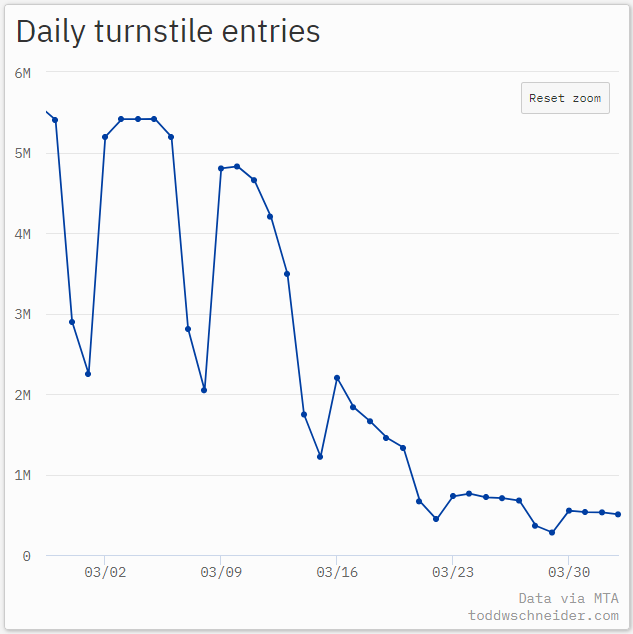
\includegraphics[width = 1.0\textwidth]{Scratch_Visuals/schneider_ridership.png}
\end{figure}
\subsection{COVID-19 in NYC}
In addition to general background knowledge about COVID-19, it would behoove the reader to know about the early spread of the disease in New York. Analysis of viral RNA in patients at the Mount Sinai Health System[\textbf{citation}] has lead researchers to conclude that the virus first came into the community through "multiple, independent but isolated introductions" from Europe and elsewhere in the USA. Below we have also given an approximate timeline of some of the most relevant events as of June 1st, 2020. We would also like to note that as forensic researchers begin examining the data, some significant new dates or corrections may arise:\\ 
\begin{itemize}
	\item February 25 - First positive test in NYC from a 39 year-old female healthcare worker flying back from Iran.
	\item March 3 - First confirmed P2P spread in NYC.
	\item March 9 - Mayor holds press conference and notes that there have been 16 confirmed cases.
	\item March 12 - Mayor declares a local state of emergency.
	\item March 15 - Schools officially close.
	\item March 22 - State order (PAUSE) to shelter in place comes into effect.
\end{itemize}
\subsection{Subway Nomenclature and Other Definitions}
\begin{itemize}
    \item {Station} - Passengers enter subway stations in order to ride the subway to an exit station.
    \item {Complex} - Multiple stations can reside in one station complex.
    \item {Turnstiles} - Barriers at the entrance and exit of stations which record people entering and exiting. 
    \item {Line} - The train tracks on which services and routes run.
    \item {Service/Route} - Trains follow specific routes between stations based on a timetable. 
    \item {Borough} - A geographical region. NYC has 5 boroughs. 
    \item {MODZCTA} - Modified Zip Code Tabulation Areas. They are very similar to zip (postal) codes, but are used due to postal codes sometimes not uniquely identifying geographical regions.
\end{itemize}
\section{Data Sources and Preprocessing}
\subsection{MTA Station Data}
This dataset has basic subway station information. It has stations, their longitude, latitude, associated complex (if any), line, route, and borough. We can find the MODZCTA from the longtitude and latitude data.\\
In this dataset, station 167 is listed twice, so we took care to combine the route data. We also split service 'S' into 3 different services as it represents 3 different shuttle services. We also split services on the 'A' line, into 3 different services depending on the destination. 
\subsection{MTA Turnstile Data}
The MTA also publishes turnstile data with turnstiles reporting every 4 hours. Prior researchers have analyzed this data down to the most specific granularity\textbf{citation needed}. However, we only need a basic picture of the daily in and out flow of each station, so we take a look at aggregate passenger flow of each station between March 1 and March 21 (inclusive). 
\subsection{NYC COVID-19 Data}
Since March 26, the NYC Health Department has been releasing and updating some COVID-19 on Github. Some data is incomplete or unavailable due to technical or privacy issues. For example, detailed case, death, and recovery numbers by MODZCTA only became available on May 18, 2020. However, a rudimentary record of positive tests for COVID-19 by modzcta has been available since April 1, 2020.
\section{Methodology}
\subsection{MESA}
To implement our ideas, we chose to use MESA, an ABM framework written in Python \textbf{citation needed}. There are many other ABM frameworks, but many of them are oriented towards beginners and lacking features to organize the code necessary for complex behavior. Others are not suitable for modeling a complex environment (network). MESA provides a simple framework with basic Agent, Model, and Schedule classes from which we can specify the necessary behavior. In addition, our group already has a working knowledge of modeling networks using Python's NetworkX, which will be necessary for specifying the environment of our model.
\subsection{Modeling Framework}
Before focusing on the NYC subways, we built a general framework for modeling various transportation problems. This allowed us to see specifically how subways (and subway commuters) differ from other types of transportation networks. It also allows us to extend our initial research into other networks and environments. In the appendix, the reader will find some other models we have built and the key point behind the modeling. Below is a UML diagram of our framework.
\begin{figure}[htbp]
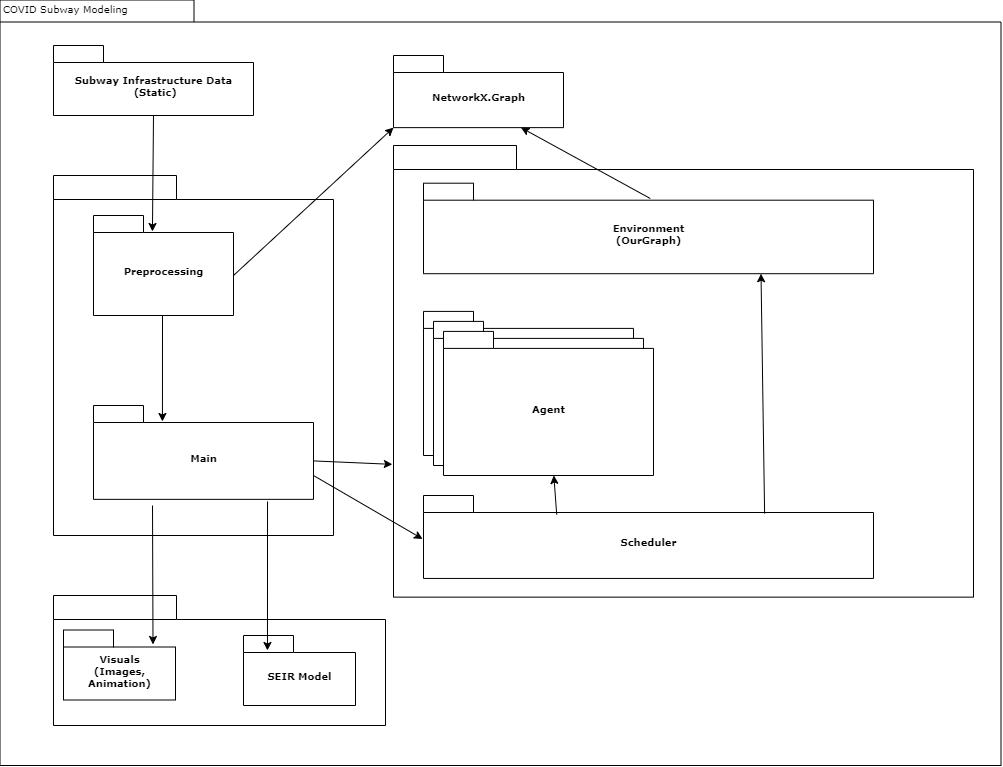
\includegraphics[width = 1.0\textwidth]{Scratch_Visuals/covid_subway.png}
\end{figure}
\subsection{SubwayModel}
\textit{...models NYC subway}
\subsubsection{SubwayAgent}
\textit{represents population using the station and surrounding areas}
\subsubsection{SubwayGraph}
\textit{represents the NYC subway. Nodes = stations, Edges = lines}
\subsection{NetworkX}
\textit{used to track the graph}
\subsection{Important Parameters and Hyper-parameters}
Hyper-parameters are capitalized and regular parameters are italicized. All parameters could be made into hyper-parameters, but we did not want to create unnecessarily complicated tuning.
\subsubsection{Basic Epidemic Characteristics}
\begin{itemize}
    \item DEFAULT\_BETA - The default $\beta$ of the modeled disease in the SEIR model. It can be affected by countermeasures. Based on research, we set this to 1.75 \textbf{citation needed}.
    \item DEFAULT\_GAMMA - The default $\gamma$ of the modeled disease in the SEIR model. It can be affected by countermeasures. Based on research, we set this to 0.50.
    \item DEFAULT\_ALPHA - The default $\alpha$ of the modeled disease in the SEIR model. It can be affected by countermeasures. Based on research, we set this to 0.20.
\end{itemize}
\subsubsection{Countermeasures}
\begin{itemize}
    \item ISOLATION\_COUNTERMEASURE - Models a government order to stay isolated after a certain number of people are infected (5000). 
    \item RECOMMENDATION\_COUNTERMEASURE - Models a government recommendation to be safe after a certain number of people are infected (500). 
    \item AWARENESS\_COUNTERMEASURE - Models increasing public awareness after a certain number of people are infected (5000). As time passes since the public first becomes aware of a problem, the infection and removal rates decrease due to self-initiative.
\end{itemize}
\subsubsection{Location-specific Characteristics}
\begin{itemize}
    \item \textit{'countermeasure defiance'} - 
    \item \textit{'exposure'} -
    \item \textit{'commute time'} -
\end{itemize}
\subsection{Algorithm}
Below is a simplified algorithm of our model.
\begin{algorithm}
\caption{Simulation of Disease Spread on Subways}\label{euclid}
\begin{algorithmic}[1]
\For{$i=1; i < TIMESPAN; i++$}
    Check conditions (i, number of infected) to see if we should deploy COUNTERMEASURES
    \For{Station in SubwayModel.Environment.Nodes}
        \State Calculate 'Local Exposure' from locally infected (and commute time).
        \State Calculate 'Route Exposure' from infected on the same route.
        \State Calculate 'General Exposure' due to city-wide infected.
        \State Update 'Exposure' At Station based on above conditions
    \EndFor
    \For{Agent in SubwayNetwork.Agents}
        \State Get 'Exposure' At Location
        \State Get City-wide COUNTERMEASURES
        \State Get Percentage of commuters
        \State Calculate SEIR beta and gamma based on conditions
        \State Update SEIR numbers
    \EndFor
\EndFor
\end{algorithmic}
\end{algorithm}
\section{Fitting}
\subsection{Fitting to SEIR}
We first fit overall SEIR numbers to NYC case, death, and recovery numbers. We only sought to fit the total cases to $I(t) + R(t)$ and adjusted the countermeasure properties to do so. Since we were at complete liberty to adjust these numbers, it is unsurprising that we created a near-perfect fit.\\
\begin{figure}[htbp]
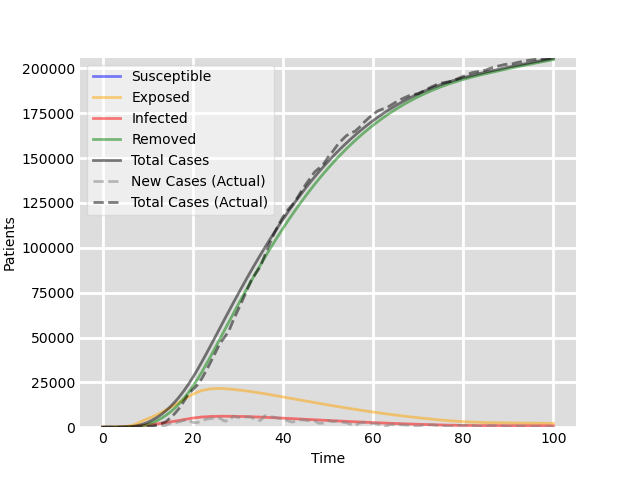
\includegraphics[width = 1.0\textwidth]{Scratch_Visuals/SEIR_Curve_NYC_3.png}
\end{figure}
\FloatBarrier
We used the following hyper-parameters:\\
\begin{itemize}
    \item RECOMMENDATION* - When 500 people are infected, divide $\beta$ and $\gamma$ by \textbf{1.5}
    \item ISOLATION** - When 5000 people are infected, divide $\beta$ by \textbf{4}, and $\gamma$ by \textbf{2}
    \item AWARENESS When 500 people are infected, $\beta$ is modified by a negative exponential function down to a minimum of 25\% of the original effect.
\end{itemize}
*Note that recommendations and isolation can be 'defied' if there are not enough infected people locally.\\
** Either the adjustment for recommendation or for isolation will take place.\\
\subsection{Fitting to MODZCTA}
Next we fit our data to MODZCTA. Due to the lack of numbers, there is no direct fitting. Also, it is difficult to visualize a timelapse in a report. Nevertheless, with some exceptions due to lack of subway coverage or missing data, our data fits actual infection hotspots very well.\\
\begin{figure}[htbp]
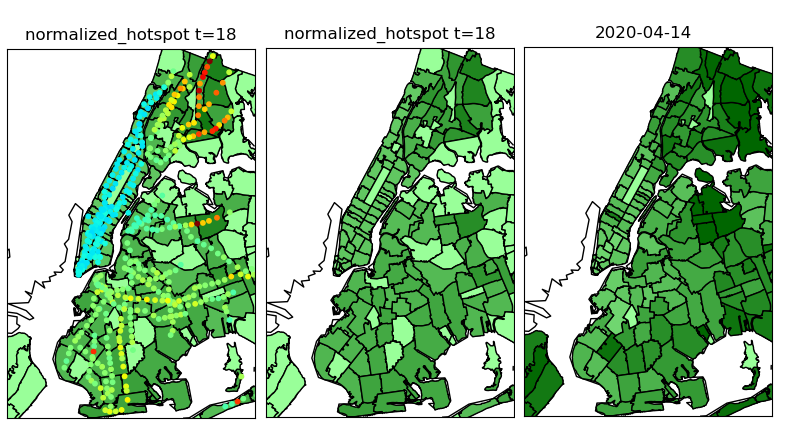
\includegraphics[width = 1.0\textwidth]{Scratch_Visuals/NYC_Geo_Fitting.png}
\end{figure}
\FloatBarrier
\textit{Scaling still TBD. Left is infected per capita (max = 0.1 percent) and Right is \textbf{total} cases per capita (max = 0.2 percent).}
\FloatBarrier
\section*{Discussion}
\textit{Measure actual difference in geographical fitting}
\textit{Countermeasures shenanigans}
\textit{Fitting on a different network. London, Singapore, Tokyo, or Moscow}
\textit{Blah blah...}
\section*{Conclusion}
\textbf{\textit{Writer's Note: All Models are Wrong, Some are Useful}}
\textit{...Predicating disease spread on subway lines, ridership at stations, commute time, and city-wide countermeasures, we were able to fit our model very closely to empirical data....}

\nocite{*}
\bibliography{bib_file}{}
\bibliographystyle{plain}
\section{Appendix}
Here be all the models that we ended up not using

\end{document}
